\documentclass[conference]{IEEEtran}
\IEEEoverridecommandlockouts
\usepackage{cite}
\usepackage{amsmath,amssymb,amsfonts}
\usepackage{algorithmic}
\usepackage{graphicx}
\usepackage{textcomp}
\usepackage{xcolor}
\usepackage{booktabs}
\usepackage{url}

\begin{document}

\title{Hybrid Mamba-Transformer Architectures for EEG-to-Text Decoding:
From Character Classification to LLM-Corrected Sentence Production}

\author{\IEEEauthorblockN{A. L. Tito}
\IEEEauthorblockA{\textit{M.Sc. Project, Department of Computer Science}\\
\textit{(placeholder affiliation --- replace before submission)}\\
email: atito@example.edu}}

\maketitle

\begin{abstract}
Decoding written language production from non-invasive brain recordings is a
central goal of brain-computer interface (BCI) research. The recent
Brain2Qwerty system showed that a convolutional front-end coupled with a
sentence-level Transformer and a character-level language model can decode
typed sentences from magneto- and electroencephalography (M/EEG), but
self-attention scales quadratically with sequence length and decoded
characters remain error-prone without strong linguistic correction. In
parallel, state-space models (SSMs) such as Mamba and Mamba-2 provide
linear-time sequence modeling, and a growing family of hybrid
Mamba-Transformer architectures (Jamba, Zamba, Hymba, Samba, Nemotron-H)
interleaves SSM and attention blocks to retain long-context accuracy at a
fraction of the cost. This paper (i) reviews the design space of hybrid
Mamba-Transformer architectures; (ii) surveys EEG decoding
architectures---EEGNet, DeepConvNet, ATCNet, EEG Conformer, EEG-Deformer,
EEGMamba, and Brain2Qwerty---for classifying characters from brain signals;
and (iii) describes a Conv + hybrid Mamba-Transformer pipeline for
M/EEG-to-text decoding in which a convolutional module feeds a
Nemotron-H-style stack of Mamba-2 blocks with periodic global attention, a
connectionist temporal classification (CTC) head produces character
sequences, a space-aware segmenter pools frames into pseudo-word embeddings
aligned to language-model space through a contrastive loss, and a
LoRA-adapted 1.1B-parameter large language model (LLM) corrects the decoded
text end to end. We compare published character-error rates across
modalities and models, analyze why the hybrid inductive bias matches the
hierarchical, sustained, and superposed neural representations measured
during language production, and specify an evaluation protocol on a
35-participant Spanish M/EEG typing dataset.
\end{abstract}

\begin{IEEEkeywords}
Brain-computer interfaces, electroencephalography (EEG),
magnetoencephalography (MEG), state-space models, Mamba-2, hybrid
Transformer, connectionist temporal classification, large language model,
brain-to-text decoding.
\end{IEEEkeywords}

\section{Introduction}
Restoring communication for patients who have lost the ability to speak or
move is one of the most impactful goals of neurotechnology. Invasive speech
and typing neuroprostheses have reached remarkable performance---for example
90 characters per minute with offline character error rates (CER) below 1\%
from intracortical handwriting signals~\cite{willett2021} and word error
rates (WER) of 9.1\% (50-word vocabulary) to 23.8\% (125,000-word
vocabulary) from intracortical speech signals~\cite{willett2023}---but they
require neurosurgery. Non-invasive decoding is far safer yet historically
much weaker: EEG letter decoding over a 10-letter alphabet was reported at a
CER of 75.8\%~\cite{crell2024}, and perception-side decoding of speech from
MEG reached 41\% top-10 accuracy over a limited
vocabulary~\cite{defossez2023}. Brain2Qwerty recently narrowed this gap by
decoding the production of briefly memorized, typed sentences from M/EEG,
reaching a CER of 32\% with MEG and 67\% with EEG using a three-stage
architecture: a convolutional module on 500~ms windows, a sentence-level
Transformer, and a pretrained 9-gram character language model (LM) that
corrects the decoded text~\cite{levy2025}.

Two bottlenecks remain in this line of work. First, the sentence-level
Transformer scales quadratically with sequence length, which limits context,
batch size, and on-device deployment for long sentences. Second, a shallow
character n-gram LM can only correct local orthographic errors; it cannot
exploit sentence-level semantics, so word-level error correction is weak
precisely where non-invasive signals are noisiest.

Meanwhile, sequence modeling has been reshaped by selective state-space
models. Mamba~\cite{gu2023mamba} and Mamba-2~\cite{dao2024ssd} match or
approach Transformer quality with linear-time recurrent inference, and
hybrid architectures that interleave a small number of attention layers into
an SSM backbone---MambaFormer~\cite{park2024mambaformer},
Jamba~\cite{lieber2024jamba}, Zamba~\cite{glorioso2024zamba},
Samba~\cite{ren2024samba}, Hymba~\cite{dong2024hymba}, and the
production-scale Nemotron-H family~\cite{nvidia2025nemotronh}---recover the
few-shot recall abilities of attention while keeping SSM efficiency. In the
EEG domain specifically, EEGMamba demonstrated that bidirectional Mamba
backbones outperform attention-based classifiers on long recordings with
linear memory growth~\cite{gui2024eegmamba}, and a foundation-model variant
pretrained Mamba encoders on large EEG corpora~\cite{wang2025eegmamba}.

This paper connects these two threads. We argue that the natural
architecture for brain-to-text decoding is a \textbf{Conv + hybrid
Mamba-Transformer}: convolutions extract local spatio-temporal features,
Mamba-2 blocks propagate information across long sentences in linear time,
sparse global attention blocks recover exact long-range alignment, and an
LLM---rather than an n-gram---performs word-level correction. The argument
is also neuroscientifically motivated: during typed language production,
letter-, syllable-, word-, and context-level representations are sustained
far beyond their execution time, superposed in population activity, and
refreshed at level-dependent speeds~\cite{zhang2025hierarchy}. A decoder
must therefore integrate local evidence over windows of very different
durations, which is precisely the regime where hybrid SSM-attention stacks
excel.

\textbf{Contributions.} (i) A structured review of hybrid Mamba-Transformer
architectures and their fusion patterns (Section~II). (ii) A comparison of
EEG character-classification architectures---EEGNet, DeepConvNet, ATCNet,
EEG Conformer, EEG-Deformer, EEGMamba, and Brain2Qwerty---emphasizing the
trade-off between local feature extraction and global sequence modeling
(Section~III). (iii) The description of a Conv + hybrid Mamba-2/attention
encoder with a CTC character head, word-level contrastive alignment, and
end-to-end LoRA-adapted LLM correction, implemented as Brain2Qwerty V3
(Section~IV). (iv) An analysis of language-model correction strategies from
n-grams to LLMs (Section~V) and a literature-anchored comparative evaluation
protocol on a Spanish M/EEG typing dataset (Section~VI).

\section{Background: State-Space Models and Hybrid Architectures}

\subsection{Structured State-Space Models and Mamba}
Continuous-time linear state-space models (SSMs) map an input signal $x(t)$
to an output $y(t)$ through a latent state $h(t)$:
\begin{equation}
\dot{h}(t) = A\,h(t) + B\,x(t), \qquad y(t) = C\,h(t)
\end{equation}
After zero-order-hold discretization with step size $\Delta$, the system
becomes a linear recurrence that can be computed either sequentially in
$O(T)$ time or as a parallel scan during training:
\begin{equation}
\bar{A} = \exp(\Delta A), \;\;
\bar{B} = (\Delta A)^{-1}(\exp(\Delta A)-I)\,\Delta B, \;\;
h_t = \bar{A}h_{t-1} + \bar{B}x_t
\end{equation}
Structured SSMs such as S4~\cite{gu2022s4} make this recurrence trainable at
scale by imposing structure on $A$. Mamba~\cite{gu2023mamba} adds a
\emph{selection mechanism}: the matrices $B$, $C$ and the step size $\Delta$
become functions of the current input,
\begin{equation}
B_t = W_B x_t, \qquad C_t = W_C x_t, \qquad
\Delta_t = \mathrm{softplus}(W_\Delta x_t + b_\Delta)
\end{equation}
so the model decides per time step what to remember or forget---a
content-aware gating that is particularly attractive for EEG, where
informative evoked responses are sparsely embedded in background noise.
Because the recurrence is time-varying, the convolutional view of S4 no
longer applies; Mamba therefore uses a hardware-aware parallel scan.

\subsection{Mamba-2 and the State-Space Duality}
Mamba-2 (structured state-space duality, SSD)~\cite{dao2024ssd} shows that
selective SSMs and masked linear attention are two parametrizations of the
same operation. The recurrence
$h_t = \exp(\Delta_t A)\,h_{t-1} + \Delta_t B_t x_t$ admits a quadratic dual
form $Y = (L \odot C B^\top) X$ (element-wise product in the mask $L$),
where the decay mask
$L[t,s] = \exp(\sum_{u=s+1}^{t} \Delta_u A)$ plays the role of a causal
attention mask with exponential forgetting. This duality is what makes
hybrid designs principled rather than ad hoc: a Mamba-2 block is attention
with a fixed, input-modulated exponential kernel, while a softmax attention
block is a data-dependent kernel without forgetting. Stacking both covers
complementary inductive biases. SSD further splits the channel dimension
into heads and shares the state across channels within a head, which raises
arithmetic intensity and allows block-decomposed (chunked) computation that
is 2--8$\times$ faster than the original selective scan while remaining
exactly recurrent at inference time~\cite{dao2024ssd}.

\subsection{Hybrid Mamba-Transformer Architectures}
Pure SSMs are efficient but weaker than attention on tasks that require
exact recall of rare token pairs, and pure attention is expensive at long
contexts. Hybrid architectures resolve this tension in several ways
(Table~\ref{tab:hybrid}). \textbf{MambaFormer}~\cite{park2024mambaformer}
interleaves Mamba and attention blocks in a single stack and shows improved
in-context learning. \textbf{Jamba}~\cite{lieber2024jamba} interleaves
Transformer and Mamba layers at a 1:7 ratio, adds mixture-of-experts MLPs,
and reaches 256K-token contexts with an 8$\times$ smaller key-value (KV)
cache than a vanilla Transformer. \textbf{Zamba}~\cite{glorioso2024zamba}
attaches a single shared global attention module every few blocks to a Mamba
backbone, amortizing attention parameters. \textbf{Samba}~\cite{ren2024samba}
combines Mamba with sliding-window attention (M-MLP-SWA-MLP repeats) and
extrapolates to 1M-token contexts. \textbf{Hymba}~\cite{dong2024hymba} fuses
attention heads and SSM heads \emph{in parallel within the same layer}
(hybrid-head), adding learnable meta tokens that act as a compressed cache.
At production scale, \textbf{Nemotron-H}~\cite{nvidia2025nemotronh} uses a
Mamba-2-majority stack with only $\sim$8\% attention blocks and reports
accuracy comparable to similarly sized Transformers with higher throughput.
Two findings from this literature matter here: (i) very few attention blocks
suffice when the SSM carries the bulk of sequence propagation, and (ii)
positional embeddings can be dropped in Mamba blocks because the recurrence
is order-aware~\cite{lieber2024jamba,nvidia2025nemotronh}.

\begin{table}[t]
\centering
\caption{Hybrid Mamba-Transformer Architectures (Language Modeling)}
\label{tab:hybrid}
\scriptsize
\begin{tabular}{@{}llll@{}}
\toprule
\textbf{Model} & \textbf{Year} & \textbf{Fusion pattern} & \textbf{Attention role} \\
\midrule
MambaFormer~\cite{park2024mambaformer} & 2024 & Interleaved Mamba/attn. & In-context recall \\
Jamba~\cite{lieber2024jamba} & 2024 & 1:7 attn.:Mamba + MoE & 1/8 of layers; 256K ctx \\
Zamba~\cite{glorioso2024zamba} & 2024 & Mamba + shared attn. & Single shared module \\
Samba~\cite{ren2024samba} & 2024 & Mamba + SWA repeats & Local recall; 1M ctx \\
Hymba~\cite{dong2024hymba} & 2024 & Parallel heads/layer & High-res.\ recall heads \\
Nemotron-H~\cite{nvidia2025nemotronh} & 2025 & Mamba-2 majority & $\sim$8\% attn.\ blocks \\
\bottomrule
\end{tabular}
\end{table}

\section{EEG Architectures for Character-Level Decoding}

\subsection{Convolutional Baselines}
CNNs remain the default inductive bias for EEG because electrode arrays are
spatially structured and evoked responses are temporally localized.
\textbf{EEGNet}~\cite{lawhern2018eegnet} packages this bias compactly: a
temporal convolution, a depthwise spatial convolution across channels, and
separable convolutions, in a few thousand parameters.
\textbf{DeepConvNet} and \textbf{ShallowConvNet}~\cite{schirrmeister2017}
generalize filter-bank decompositions with deeper convolutional stacks.
These models excel at short segments but have a bounded receptive field and
no mechanism for sentence-level context, which limits them in typed-text
decoding: in Brain2Qwerty's comparison, EEGNet was 1.14$\times$ worse (EEG)
and 2.25$\times$ worse (MEG) in CER than the full Conv+Transformer+LM
model~\cite{levy2025}.

\subsection{Convolution-Transformer Hybrids}
\textbf{EEG Conformer}~\cite{song2023conformer} is the canonical
conv-transformer for EEG: a convolutional module extracts local temporal and
spatial features, and a self-attention encoder captures global correlations,
reaching 78.66\% (BCI Competition IV-2a, hold-out), 84.63\% (IV-2b) and
95.30\% (SEED) in its original evaluation. \textbf{ATCNet}~\cite{altaheri2023atcnet}
augments a temporal convolutional network with multi-head attention for
motor imagery. \textbf{EEG-Deformer}~\cite{ding2024deformer} adds dense
coarse-to-fine temporal branches to the Conformer pattern, improving over
EEG Conformer by 2.9--5.0 percentage points across attention, fatigue, and
workload classification. The consistent lesson of this family is that
convolutions plus attention beat either alone---but all of them inherit the
$O(T^2)$ cost and KV-cache growth of softmax attention, and all are trained
as isolated classifiers rather than as the front-end of a text production
pipeline.

\subsection{State-Space EEG Models}
\textbf{EEGMamba}~\cite{gui2024eegmamba} was the first architecture to bring
selective SSMs to EEG classification: a spatio-temporal-adaptive tokenizer,
bidirectional Mamba blocks (necessary because offline EEG analysis is
non-causal), and a task-aware mixture of experts. Across eight public
datasets spanning seizure detection, emotion recognition, sleep staging, and
motor imagery it outperformed EEGNet, AttnSleep, and EEG Conformer on most
benchmarks, while memory grows linearly with signal length---handling
sequences beyond 40,000 samples where attention baselines approach
out-of-memory~\cite{gui2024eegmamba}. A successor scaled the idea into an
EEG foundation model with patch-based masked reconstruction
pretraining~\cite{wang2025eegmamba}. These results establish that SSMs are
competitive with attention on EEG; what they do not address is
open-vocabulary text production, which additionally requires character-level
alignment (CTC-style) and linguistic correction.

\subsection{Brain2Qwerty: Brain-to-Text via Typing}
\textbf{Brain2Qwerty}~\cite{levy2025} is the reference point for this paper.
Thirty-five healthy participants read Spanish sentences presented word by
word (rapid serial visual presentation), memorized them during a 1.5~s
fixation, and typed them from memory without visual feedback, while
306-channel MEG and/or 64-channel EEG were recorded. The decoder combines
(1) a convolutional module with a subject-specific linear layer applied to
500~ms windows, (2) a sentence-level Transformer over the pooled window
embeddings, and (3) a pretrained 9-gram character LM applied at decoding.
Trained end-to-end (about 400M parameters: 258M convolutional + 138M
Transformer), it reaches CER = 32~$\pm$~0.6\% (MEG) and 67~$\pm$~1.5\%
(EEG), with the best participant at 19\% CER on MEG and several perfectly
decoded held-out sentences~\cite{levy2025}. Ablations show each stage
contributes: the conv module alone already beats EEGNet, the Transformer
improves CER significantly, and the LM improves it further. The companion
neuroscience analysis~\cite{zhang2025hierarchy} shows that during typing,
context-, word-, syllable-, and letter-level representations rise in
top-down order and are each sustained much longer than their execution time
(letters: about 103~ms keypresses decodable for over 1~s; context sustained
for seconds), with up to five successive letters simultaneously
decodable---direct evidence that a brain-to-text decoder faces a long,
superposed, multi-scale temporal integration problem.

\begin{table}[t]
\centering
\caption{EEG Architectures Relevant to Character-Level Decoding}
\label{tab:eeg}
\scriptsize
\begin{tabular}{@{}lllll@{}}
\toprule
\textbf{Model} & \textbf{Year} & \textbf{Sequence core} & \textbf{Global} & \textbf{Scaling} \\
\midrule
EEGNet~\cite{lawhern2018eegnet} & 2018 & Depthwise/sep.\ CNN & None & $O(T)$ \\
DeepConvNet~\cite{schirrmeister2017} & 2017 & Deep CNN & None & $O(T)$ \\
ATCNet~\cite{altaheri2023atcnet} & 2023 & Attention + TCN & Attn.\ over TCN & $O(T^2)$ \\
EEG Conformer~\cite{song2023conformer} & 2023 & Conv + Transformer & Full attn. & $O(T^2)$ \\
EEG-Deformer~\cite{ding2024deformer} & 2024 & Dense conv-Transf. & Full attn. & $O(T^2)$ \\
EEGMamba~\cite{gui2024eegmamba} & 2024 & Bi-Mamba + MoE & Selective SSM & $O(T)$ \\
Brain2Qwerty~\cite{levy2025} & 2025 & Conv+Transf.+9-gram & Full attn. & $O(T^2)$ \\
\textbf{Ours (B2Q V3)} & 2026 & Conv + hybr.\ M-2/attn. + LLM & SSM + sparse & mostly $O(T)$ \\
\bottomrule
\end{tabular}
\end{table}

\section{Proposed Conv + Hybrid Mamba-Transformer Pipeline}

\subsection{Overview}
The proposed architecture (Fig.~\ref{fig:arch}), implemented as Brain2Qwerty
V3, replaces the sentence-level Transformer of Brain2Qwerty with a
Nemotron-H-style hybrid Mamba-2/attention stack~\cite{nvidia2025nemotronh}
and replaces the shallow 9-gram corrector with an end-to-end LoRA-adapted
LLM~\cite{hu2022lora}. Five modules share one encoder forward pass: (i) a
convolutional front-end; (ii) the hybrid sequence core; (iii) a CTC
character head with auxiliary supervision; (iv) a CTC space-based word
segmenter whose pooled word embeddings are aligned to the LLM's embedding
space by a contrastive loss; and (v) a frozen 1.1B-parameter
LLM~\cite{llama3} with LoRA adapters (0.05\% trainable parameters) that
generates the corrected sentence conditioned on both the greedy CTC
transcript and the neural word embeddings. The total objective is
\begin{equation}
\mathcal{L} = w_{\mathrm{ctc}}\,\mathcal{L}_{\mathrm{CTC}}
+ w_{\mathrm{con}}\,\mathcal{L}_{\mathrm{con}}
+ w_{\mathrm{llm}}\,\mathcal{L}_{\mathrm{LM}}
\end{equation}
with weights $(1-\alpha-\beta,\ \alpha,\ \beta)$, $\alpha=0.1$, $\beta=0.01$
by default, gated by epoch so that each loss can be phased in after the
encoder has stabilized.

\subsection{Convolutional Front-End}
Following the Brain2Qwerty design~\cite{levy2025} and the subject layer of
D\'efossez et al.~\cite{defossez2023}, each 500~ms M/EEG window (band-passed
0.5--45~Hz, notch-filtered at line-noise harmonics, downsampled) is linearly
remapped by a subject-specific layer that learns a per-participant spatial
montage, followed by spatial and temporal convolutions with downsampling.
The output is a sequence of window embeddings at a reduced frame rate, short
enough that a handful of attention blocks is cheap, yet long enough that the
SSM blocks carry the bulk of temporal propagation. This division of
labor---convolutions for local spatio-temporal features, SSM for long-range
integration---mirrors the evidence that conv+sequence hybrids dominate pure
CNNs and pure Transformers on EEG~\cite{song2023conformer,ding2024deformer}.

\subsection{Hybrid Mamba-2/Attention Sequence Core}
The sequence core stacks $N=8$ pre-norm residual blocks in the pattern
[M, M, M, A, M, M, M, A] (one attention block every four), followed by a
final RMSNorm. Each Mamba-2 block applies the SSD mixer: an input projection
produces the gate $z$, the conv branch $[x, B, C]$, and the step-size
logits; a causal depthwise convolution (kernel 4) with SiLU pre-smooths the
branch---acting as a learned local filter against high-frequency EEG
artifacts---and the selective recurrence
\begin{equation}
h_t = \exp(\Delta_t A)\,h_{t-1} + \Delta_t B_t x_t, \qquad
y_t = C_t h_t + D\,x_t
\end{equation}
is evaluated in its quadratic dual form (Section~II-B) computed in float32
and chunked over heads to bound memory. The output passes through a gated
RMSNorm (gate applied as $x * \mathrm{silu}(z)$ before the norm, matching
the reference implementation) and an output projection. Attention blocks are
single encoder layers with rotary position embeddings~\cite{su2021roformer},
RMSNorm, four heads, and a small feed-forward sublayer. No positional
information is added to Mamba blocks, since the recurrence is
order-aware~\cite{lieber2024jamba}. With the frame rate produced by the conv
front-end (a few hundred frames per sentence), the 75\% of blocks that are
SSM run in $O(T)$, and only the two attention blocks pay the quadratic cost;
Fig.~\ref{fig:results}(a) illustrates the scaling argument. The encoder
totals approximately 358M trainable parameters---comparable to the
Brain2Qwerty Conv+Transformer, so any gain can be attributed to architecture
rather than scale.

\subsection{CTC Character Decoding}
Because keypress timings within the continuous typing stream are only
partially aligned with neural responses, the character head is trained with
connectionist temporal classification (CTC)~\cite{graves2006ctc}, which
marginalizes over all alignments $\pi$ between encoder frames and the target
character sequence $y$:
\begin{equation}
\mathcal{L}_{\mathrm{CTC}} = -\log \sum_{\pi \in \mathcal{B}^{-1}(y)}
\prod_t p(\pi_t \mid X)
\end{equation}
An auxiliary CTC head on an intermediate representation is blended with the
final head (30\% final, 70\% auxiliary by default), which stabilizes
training of the deep hybrid stack. At inference, greedy CTC decoding yields
a raw character transcript (e.g.\ `stamistosasigue la distribucion').

\subsection{Word Segmentation and Contrastive Alignment}
To move from characters to words, predicted space characters in the CTC
posteriors define boundaries; encoder frames between successive spaces
(including blank frames) are mean-pooled by a small trainable pooler into
one pseudo-word embedding per hypothesized word. A projection adapter maps
these embeddings into the LLM's word-embedding space, where a word-level
contrastive loss pulls each neural word embedding toward the text embedding
of the true word (computed once by the frozen LLM) and away from the other
words in the batch. This gives the encoder a word-level training signal that
CTC---a purely character-level objective---cannot provide, and it is what
makes the neural word embeddings interpretable to the LLM at correction
time.

\subsection{LLM-Based Word Correction}
The final stage replaces the 9-gram character LM of
Brain2Qwerty~\cite{levy2025} with a LoRA-adapted~\cite{hu2022lora}
instruction-tuned LLM (1.1B parameters, frozen base; 563K trainable adapter
parameters plus a 2.1M projection adapter). The model receives a prefix
built in embedding space: the tokenized greedy CTC transcript (``CTC:
\ldots''), followed by the adapted neural word embeddings (``MEG:
\ldots''), and a response marker (``Output:''), and is trained with
teacher-forced cross-entropy (label smoothing 0.02) to generate the true
sentence. At inference, beam search (16 beams, length penalty 0.2) produces
the corrected sentence. Because the LLM sees both a noisy character
transcript and a word-level neural representation, it can arbitrate between
them: character errors that would defeat a character n-gram (e.g.\ `EK
BENEFUCU SYOERA KIS RUESGIS' for `el beneficio supera los riesgos') are
exactly the regime where a pretrained LLM's lexical and syntactic priors are
strongest~\cite{levy2025,caria2025}. Modality dropout on both the neural
embeddings and the CTC text during training prevents the LLM from ignoring
the neural input.

\begin{figure}[t]
\centering
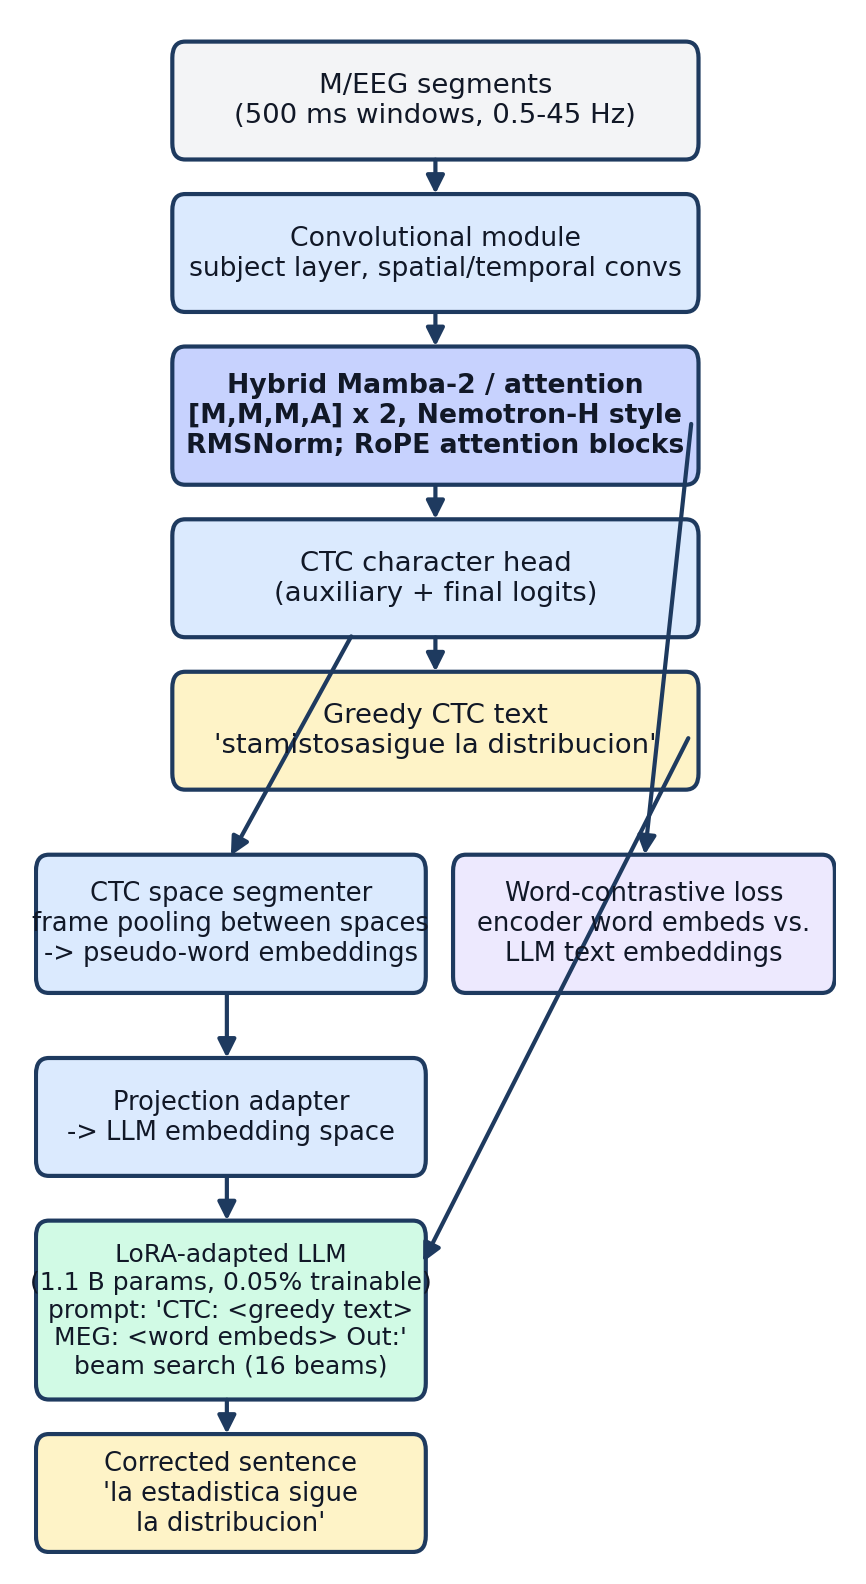
\includegraphics[width=\columnwidth]{fig_architecture.png}
\caption{Proposed Conv + hybrid Mamba-Transformer brain-to-text pipeline
(Brain2Qwerty V3). A convolutional front-end feeds a Nemotron-H-style stack
of Mamba-2 blocks with periodic attention; a CTC head yields character
sequences; a space-based segmenter pools frames into pseudo-word embeddings
aligned to LLM space by a contrastive loss; a LoRA-adapted LLM generates the
corrected sentence.}
\label{fig:arch}
\end{figure}

\section{Language-Model Correction Strategies for Brain-to-Text}
Neural decoders and language models play complementary roles: the decoder
maps brain activity to symbols, and the LM enforces linguistic plausibility.
Four strategies exist, in increasing order of LM capacity
(Table~\ref{tab:lm}). (1) \textbf{Character n-gram fusion}: Brain2Qwerty
rescores CTC outputs with a pretrained 9-gram character LM~\cite{levy2025},
similar in spirit to the 5-gram decoders used in invasive speech
BCIs~\cite{willett2023}. n-grams are cheap and robust, but their short
context cannot model semantics. (2) \textbf{LLM rescoring}: n-best
hypotheses from the decoder are rescored by a pretrained LLM; in speech BCI
pipelines, adding conversational context to OPT- or GPT-2-scale rescoring
reduced both CER and WER by roughly 2 absolute points relative to
n-gram-only decoding~\cite{willett2023}. (3) \textbf{Sequence-to-sequence
translation}: DeWave maps discrete EEG codex tokens to text with a BART
encoder-decoder~\cite{duan2024dewave}, building on open-vocabulary
EEG-to-text with pretrained LM priors~\cite{wang2022eeg2text}; this works
for reading-evoked EEG but entangles alignment and correction in a single
black box. (4) \textbf{End-to-end conditioned LLM} (ours): the LLM is
fine-tuned with LoRA to read both the noisy transcript and the neural word
embeddings, so correction is trained jointly with the encoder and can
exploit information that never survives greedy character decoding---an
approach consistent with the broader trend of fusing LLMs into BCI spellers
for word prediction, completion, and error correction~\cite{caria2025}. The
Word Error Rate (WER) and semantic error metrics (SemER) are the natural
evaluation criteria at this stage.

\begin{table}[t]
\centering
\caption{Language-Model Correction Strategies for Brain-to-Text}
\label{tab:lm}
\scriptsize
\begin{tabular}{@{}llll@{}}
\toprule
\textbf{Strategy} & \textbf{Example} & \textbf{Strength} & \textbf{Weakness} \\
\midrule
Char.\ n-gram fusion & B2Q 9-gram~\cite{levy2025} & Cheap, robust & No semantics \\
LLM rescoring & OPT/GPT-2~\cite{willett2023} & No retraining & n-best limited \\
Seq2seq translation & DeWave~\cite{duan2024dewave} & Open vocab. & Entangled \\
\textbf{E2E LoRA LLM} & B2Q V3~\cite{hu2022lora} & Sees neural embeds & Heavier \\
\bottomrule
\end{tabular}
\end{table}

\section{Experimental Setup and Comparative Analysis}

\subsection{Dataset and Task}
Experiments use the Spanish read-wait-type dataset recorded at the Basque
Center on Cognition, Brain and Language (BCBL)~\cite{levy2025,zhang2025hierarchy}:
35 healthy native Spanish speakers (20 MEG, 20 EEG, 5 both), 128 unique
declarative sentences of 5--8 words, MEG at 306 channels (1~kHz, online
0.1--330~Hz) and EEG at 61+3 channels, preprocessed to 0.5--45~Hz and
downsampled. Each trial consists of RSVP reading, a 1.5~s wait, and
memory-guided typing with no visual letter feedback. Typographical errors
are filtered by Levenshtein alignment between the displayed and typed
sentences.

\subsection{Metrics}
Character error rate CER = $(S+D+I)/N$ (substitutions, deletions, insertions
over sentence length) is the primary metric, following the ASR convention
adopted in brain-to-text work~\cite{levy2025,willett2021}; word error rate
(WER) and SemER evaluate the corrected output. Statistical comparisons
across subjects use Wilcoxon signed-rank tests, as in the reference study.

\subsection{Literature-Reported Comparison}
Fig.~\ref{fig:results}(b) and Table~\ref{tab:results} collect the published
reference points. Non-invasive letter decoding without a sentence context is
weak: Crell and M\"uller-Putz report 75.8\% CER over a 10-letter EEG
alphabet~\cite{crell2024}. Sentence-level decoding with a deep pipeline
changes the picture: Brain2Qwerty reaches 67\% CER on EEG and 32\% on MEG,
and 19\% for the best MEG participant---at which point some held-out
sentences are decoded perfectly~\cite{levy2025}. For calibration, invasive
systems remain well ahead: 9.1\% WER (50-word) and 23.8\% WER
(125,000-word) for intracortical speech~\cite{willett2023}, 15.2\% CER at 79
words per minute for ECoG speech~\cite{metzger2023}, and under 1\% offline
CER for intracortical handwriting with a correction model~\cite{willett2021}.
Two implications follow: the sensor modality contributes about a 2$\times$
CER gap (MEG vs.\ EEG), and architecture plus language modeling contributes
a comparable factor within a modality---the Conv+Transformer+LM pipeline
improves CER 1.14$\times$ (EEG) and 2.25$\times$ (MEG) over EEGNet, and
ablations show the Transformer and the LM each add significant
gains~\cite{levy2025}.

\subsection{Expected Benefits of the Hybrid Design and Evaluation Protocol}
The proposed V3 pipeline is currently being trained on the Spanish BCBL
dataset; consequently, we do not report new empirical numbers and instead
state the hypotheses the design targets. \textbf{H1 (efficiency):} at equal
parameters ($\sim$358M), replacing 75\% of attention blocks with Mamba-2
reduces memory and increases throughput for sentence-length sequences,
following the scaling behavior measured for SSM EEG
backbones~\cite{gui2024eegmamba} and hybrid
LLMs~\cite{lieber2024jamba,nvidia2025nemotronh}. \textbf{H2 (accuracy):} the
selective SSM's input-dependent gating should track the sustained,
superposed letter/word representations documented in the companion
neuroscience study~\cite{zhang2025hierarchy} better than full attention at
equal compute, because exponential decay with selective gating matches the
measured dynamic-code structure. \textbf{H3 (correction):} end-to-end
LoRA-adapted LLM correction should reduce WER beyond the 9-gram LM of the
reference system, particularly on rare and out-of-vocabulary words, where
n-gram priors are weakest~\cite{levy2025,caria2025}. The evaluation protocol
mirrors Brain2Qwerty: per-subject and pooled models, held-out sentences,
Wilcoxon tests against the V2 Conv+Transformer+9-gram baseline, ablations
removing attention blocks, the contrastive loss, and the LLM stage, and
complexity benchmarks (memory and latency vs.\ sentence length).

\begin{figure}[t]
\centering
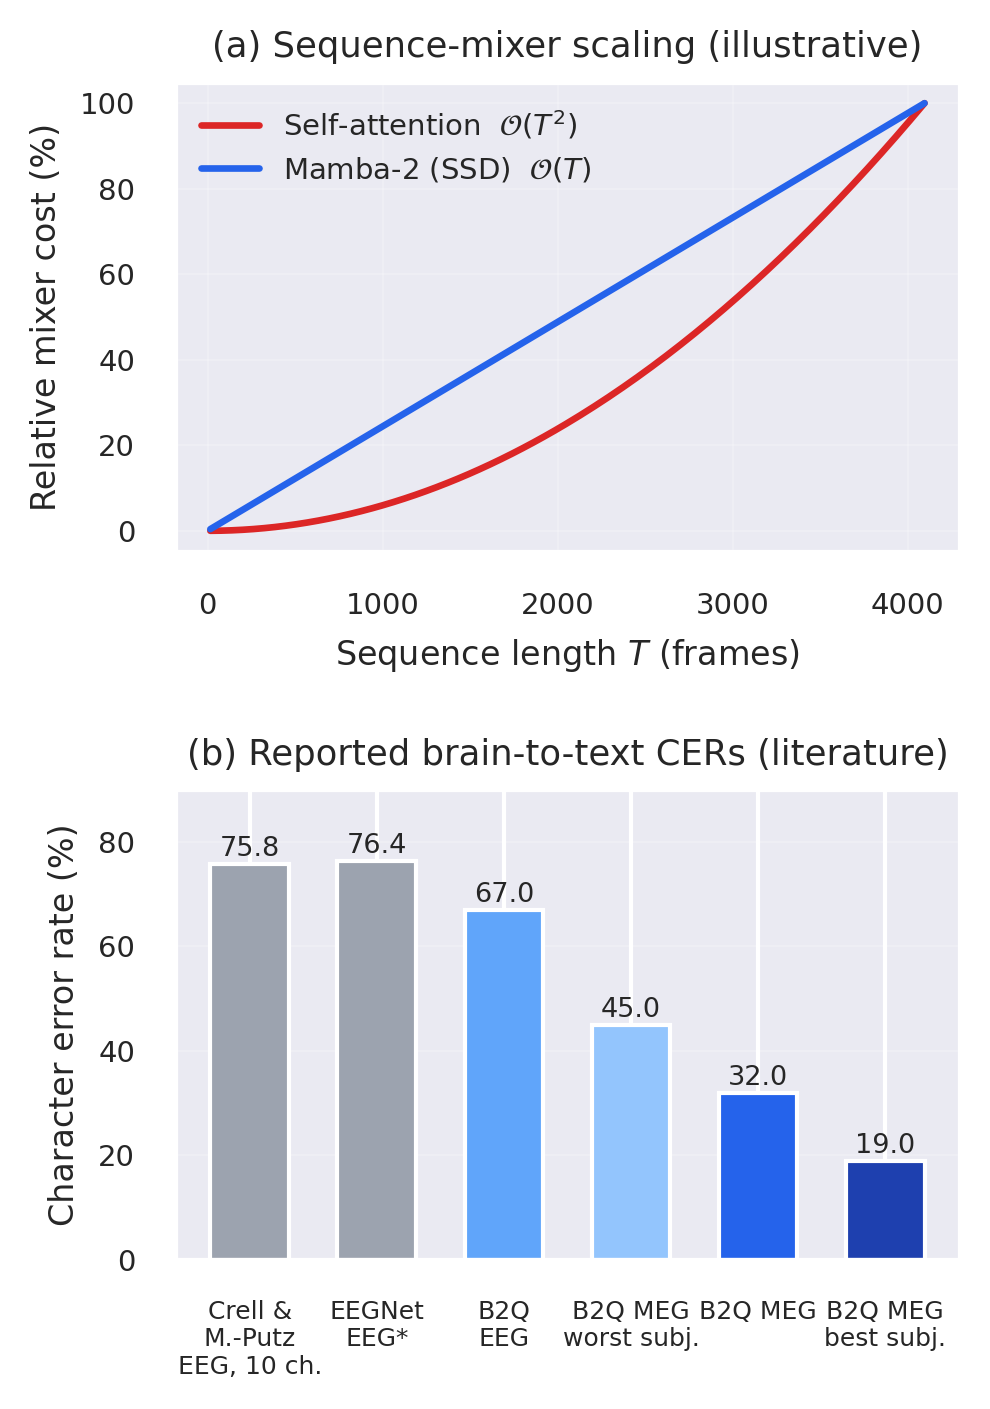
\includegraphics[width=\columnwidth]{fig_results.png}
\caption{(a) Illustrative scaling of the sequence mixer: softmax attention
grows quadratically in sequence length, while the Mamba-2 SSD recurrence
grows linearly~\cite{gu2023mamba,dao2024ssd}. (b) Published brain-to-text
character error rates~\cite{levy2025,crell2024}. B2Q = Brain2Qwerty.
$^*$As reported in~\cite{levy2025}. $^\dagger$Derived from the reported
1.14$\times$ CER improvement of the full Brain2Qwerty model over EEGNet on
EEG.}
\label{fig:results}
\end{figure}

\begin{table}[t]
\centering
\caption{Reported Brain-to-Text / Typing Decoding Performance}
\label{tab:results}
\scriptsize
\begin{tabular}{@{}llll@{}}
\toprule
\textbf{System} & \textbf{Modality} & \textbf{Task} & \textbf{Reported error} \\
\midrule
Crell \& M.-Putz~\cite{crell2024} & EEG & 10-letter classif. & 75.8\% CER$^*$ \\
EEGNet~\cite{lawhern2018eegnet,levy2025} & EEG & Sentence typing & $\sim$76\% CER$^\dagger$ \\
Brain2Qwerty~\cite{levy2025} & EEG & Sentence typing & 67 $\pm$ 1.5\% CER \\
Brain2Qwerty~\cite{levy2025} & MEG & Sentence typing & 32 $\pm$ 0.6\% (best 19\%) \\
Willett 2021~\cite{willett2021} & Intracortical & Handwriting & $<$1\% CER (offline) \\
Willett 2023~\cite{willett2023} & Intracortical & Speech & 9.1\%/23.8\% WER \\
Metzger 2023~\cite{metzger2023} & ECoG & Speech & 15.2\% CER, 79 wpm \\
\bottomrule
\end{tabular}
\end{table}

\section{Discussion}
\textbf{Why hybrids fit brain-to-text.} The measured neural code of typing
is hierarchical and superposed: fast, dynamic letter codes co-exist with
slow, sustained context codes~\cite{zhang2025hierarchy}. Convolutional
layers match the fast motor-somatosensory transients; Mamba-2's
input-dependent decay implements multi-scale memory in a single block type,
with different heads learning different time constants through the step-size
parameter; and sparse attention blocks recover exact alignment when a
distant frame must be compared directly---the same reason hybrids dominate
pure SSMs on recall-heavy language
tasks~\cite{dong2024hymba,park2024mambaformer}.

\textbf{Practicality.} The hybrid stack keeps the parameter count of the
Transformer baseline while moving most sequence computation into
linear-time blocks, and the LoRA correction stage adds only $\sim$0.05\%
trainable parameters over a frozen 1.1B model---the entire system trains in
bfloat16 on commodity GPUs. Because only the correction stage requires the
LLM at inference, latency-critical online decoding can still use greedy CTC
output while the LLM refines text at sentence boundaries.

\textbf{Limitations.} (i) Non-invasive decoding remains motor-dominated:
error analyses in the reference study show decoding relies substantially on
motor processes, so applicability to non-typing patients (the clinical
target) is unproven~\cite{levy2025}. (ii) The dataset is small (35
participants, 128 sentences), and hybrid LLM findings may not transfer at
this scale. (iii) Our implementation evaluates the SSD dual form in its
quadratic mode; the memory benefit of the chunked scan is realized only at
longer contexts. (iv) LLM correction can hallucinate fluent but wrong
sentences, so CER/WER must be reported alongside semantic metrics, and
high-stakes use needs conservative operating points~\cite{caria2025}.
(v) Causality: for real-time use the bidirectional/non-causal components
must be restricted, echoing the distinction EEGMamba draws between offline
and online settings~\cite{gui2024eegmamba}.

\textbf{Future work.} Promising directions include bidirectional Mamba-2
variants for offline decoding~\cite{gui2024eegmamba}, pretraining the
encoder on large unlabeled EEG corpora in the style of EEG foundation
models~\cite{wang2025eegmamba}, scaling data collection (the reference study
found CER improves log-linearly with recording time~\cite{levy2025}),
cross-subject transfer through the subject layer, and unifying the LLM
correction with conversational context as in rescoring-based speech BCI
pipelines~\cite{willett2023}.

\section{Conclusion}
Hybrid Mamba-Transformer architectures reconcile the two dominant
sequence-model paradigms: SSMs give linear-time, order-aware propagation
with multi-scale forgetting, while sparse attention restores exact global
recall. For EEG-to-text decoding, this combination maps naturally onto the
hierarchical, sustained, and superposed neural representations of language
production. The presented Conv + hybrid Mamba-2/attention
pipeline---convolutional front-end, Nemotron-H-style core, CTC character
head, contrastively aligned word embeddings, and LoRA-adapted LLM
correction---upgrades every stage of the Brain2Qwerty reference architecture
at comparable parameter count, and defines a concrete, testable path toward
accurate non-invasive brain-to-text systems. The literature comparison
underscores the stakes: closing even part of the gap between the 32\% MEG
CER of current non-invasive decoding and the single-digit error rates of
invasive neuroprostheses would mark a qualitative step toward safe
communication BCIs.

\begin{thebibliography}{33}
\bibitem{vaswani2017} A. Vaswani, N. Shazeer, N. Parmar, J. Uszkoreit,
L. Jones, A. N. Gomez, L. Kaiser, and I. Polosukhin, ``Attention is all you
need,'' in \emph{Proc. NeurIPS}, 2017.
\bibitem{gu2022s4} A. Gu, K. Goel, and C. R\'e, ``Efficiently modeling long
sequences with structured state spaces,'' in \emph{Proc. ICLR}, 2022.
\bibitem{gu2023mamba} A. Gu and T. Dao, ``Mamba: Linear-time sequence
modeling with selective state spaces,'' in \emph{Proc. COLM}, 2024,
arXiv:2312.00752.
\bibitem{dao2024ssd} T. Dao and A. Gu, ``Transformers are SSMs: Generalized
models and efficient algorithms through structured state space duality,'' in
\emph{Proc. ICML}, 2024.
\bibitem{lieber2024jamba} O. Lieber, B. Lenz, H. Bata, G. Cohen, J. Osin,
I. Dalmedigos, et al., ``Jamba: A hybrid transformer-mamba language model,''
arXiv:2403.19887, 2024.
\bibitem{glorioso2024zamba} P. Glorioso, Q. Anthony, Y. Tokpanov,
J. Whittington, J. Pilault, A. Ibrahim, and B. Millidge, ``Zamba: A compact
7B SSM hybrid model,'' arXiv:2405.16712, 2024.
\bibitem{dong2024hymba} X. Dong, Y. Fu, S. Diao, W. Byeon, Z. Chen,
A. S. Mahabaleshwarkar, et al., ``Hymba: A hybrid-head architecture for
small language models,'' arXiv:2411.13676, 2024.
\bibitem{ren2024samba} L. Ren, Y. Liu, Y. Lu, Y. Shen, C. Liang, and
W. Chen, ``Samba: Simple hybrid state space models for efficient unlimited
context language modeling,'' arXiv:2406.07522, 2024.
\bibitem{park2024mambaformer} J. Park, J. Park, Z. Xiong, N. Lee, J. Cho,
S. Oymak, K. Lee, and D. Papailiopoulos, ``Can Mamba learn how to learn? A
comparative study on in-context learning tasks,'' in \emph{Proc. ICML}, 2024.
\bibitem{nvidia2025nemotronh} NVIDIA, ``Nemotron-H: A family of accurate and
efficient hybrid mamba-transformer models,'' arXiv:2504.03624, 2025.
\bibitem{lawhern2018eegnet} V. J. Lawhern, A. J. Solon, N. R. Waytowich,
S. M. Gordon, C. P. Hung, and B. J. Lance, ``EEGNet: a compact convolutional
neural network for EEG-based brain-computer interfaces,'' \emph{J. Neural
Eng.}, vol. 15, no. 5, 2018.
\bibitem{schirrmeister2017} R. T. Schirrmeister et al., ``Deep learning with
convolutional neural networks for EEG decoding and visualization,''
\emph{Human Brain Mapping}, vol. 38, no. 11, 2017.
\bibitem{song2023conformer} Y. Song, Q. Zheng, B. Liu, and X. Gao, ``EEG
Conformer: Convolutional transformer for EEG decoding and visualization,''
\emph{IEEE Trans. Neural Syst. Rehabil. Eng.}, vol. 31, pp. 710--719, 2023.
\bibitem{ding2024deformer} J. Ding, Y. Li, Z. Jiang, and D. Wu,
``EEG-Deformer: A dense convolutional transformer for brain-computer
interfaces,'' arXiv:2405.00719, 2024.
\bibitem{altaheri2023atcnet} H. Altaheri, G. Muhammad, M. Alsulaiman,
S. U. Amin, G. A. Altuwaijri, W. Abdul, M. A. Bencherif, and M. Faisal,
``Physics-informed attention temporal convolutional network for EEG-based
motor imagery classification,'' \emph{IEEE Trans. Ind. Informat.}, vol. 19,
no. 2, pp. 2249--2258, 2023.
\bibitem{gui2024eegmamba} Y. Gui, M. Chen, Y. Su, G. Luo, and Y. Yang,
``EEGMamba: Bidirectional state space models with mixture of experts for EEG
classification,'' arXiv:2407.20254, 2024.
\bibitem{wang2025eegmamba} J. Wang, S. Zhao, Z. Luo, Y. Zhou, S. Li, and
G. Pan, ``EEGMamba: An EEG foundation model with Mamba,'' \emph{Neural
Networks}, 107816, 2025.
\bibitem{levy2025} J. L\'evy, M. Zhang, S. Pinet, J. Rapin, H. Banville,
S. d'Ascoli, and J.-R. King, ``Brain-to-text decoding: A non-invasive
approach via typing,'' arXiv:2502.17480, 2025.
\bibitem{zhang2025hierarchy} M. Zhang, J. L\'evy, S. d'Ascoli, J. Rapin,
F.-X. Alario, P. Bourdillon, S. Pinet, and J.-R. King, ``A hierarchy of
dynamic neural codes coordinates the production of language,''
arXiv:2502.07429, 2025.
\bibitem{defossez2023} C. D\'efossez, C. Caucheteux, J. Rapin, O. Kabeli,
and J.-R. King, ``Decoding speech perception from non-invasive brain
recordings,'' \emph{Nature Machine Intelligence}, vol. 5, pp. 912--921,
2023.
\bibitem{willett2021} F. R. Willett, D. T. Avansino, L. R. Hochberg,
J. M. Henderson, and K. V. Shenoy, ``High-performance brain-to-text
communication via handwriting,'' \emph{Nature}, vol. 593, pp. 249--254,
2021.
\bibitem{willett2023} F. R. Willett, E. M. Kunz, C. Fan, D. T. Avansino,
G. H. Wilson, E. Y. Choi, F. Kamdar, M. F. Glasser, L. R. Hochberg,
S. Druckmann, K. V. Shenoy, and J. M. Henderson, ``A high-performance speech
neuroprosthesis,'' \emph{Nature}, vol. 620, pp. 1031--1036, 2023.
\bibitem{metzger2023} S. L. Metzger, K. T. Littlejohn, A. B. Silva,
D. A. Moses, M. P. Seaton, R. Wang, et al., ``A high-performance
neuroprosthesis for speech decoding and avatar control,'' \emph{Nature},
vol. 620, pp. 1037--1046, 2023.
\bibitem{duan2024dewave} Y. Duan, J. Zhou, Z. Wang, Y.-K. Wang, and C.-T.
Lin, ``DeWave: Discrete EEG waves encoding for brain dynamics to text
translation,'' in \emph{Proc. NeurIPS}, 2023.
\bibitem{wang2022eeg2text} Z. Wang and H. Ji, ``Open vocabulary
electroencephalography-to-text decoding and zero-shot sentiment
classification,'' in \emph{Proc. AAAI}, vol. 36, pp. 5350--5358, 2022.
\bibitem{graves2006ctc} A. Graves, S. Fern\'andez, F. Gomez, and
J. Schmidhuber, ``Connectionist temporal classification: Labelling
unsegmented sequence data with recurrent neural networks,'' in \emph{Proc.
ICML}, 2006.
\bibitem{hu2022lora} E. J. Hu, Y. Shen, P. Wallis, Z. Allen-Zhu, Y. Li,
S. Wang, L. Wang, and W. Chen, ``LoRA: Low-rank adaptation of large language
models,'' in \emph{Proc. ICLR}, 2022.
\bibitem{king2014} J.-R. King and S. Dehaene, ``Characterizing the dynamics
of mental representations: The temporal generalization method,''
\emph{Trends in Cognitive Sciences}, vol. 18, no. 4, pp. 203--210, 2014.
\bibitem{crell2024} M. R. Crell and G. R. M\"uller-Putz, ``Handwritten
character classification from EEG through continuous kinematic decoding,''
\emph{J. Neural Eng.}, 2024.
\bibitem{tang2023} J. Tang, A. LeBel, S. Jain, and A. G. Huth, ``Semantic
reconstruction of continuous language from non-invasive brain recordings,''
\emph{Nature Neuroscience}, vol. 26, pp. 858--866, 2023.
\bibitem{caria2025} A. Car\`ia et al., ``Towards predictive communication:
The fusion of large language models and brain-computer interface,'' 2025.
\bibitem{llama3} A. Grattafiori, A. Dubey, A. Jauhri, et al., ``The Llama 3
herd of models,'' arXiv:2407.21783, 2024.
\bibitem{su2021roformer} J. Su, M. Ahmed, Y. Lu, S. Pan, W. Bo, and Y. Liu,
``RoFormer: Enhanced transformer with rotary position embedding,''
arXiv:2104.09864, 2021.
\end{thebibliography}

\end{document}
